\chapter{Environment}
\label{chapter:environment}

Kata Containers background \\
Different partitions of KC \\
Our environment \\
Usage of KC in our environment \\

\begin{figure}[ht]
  \begin{center}
    % here the width of the figure is set to 9 cm
    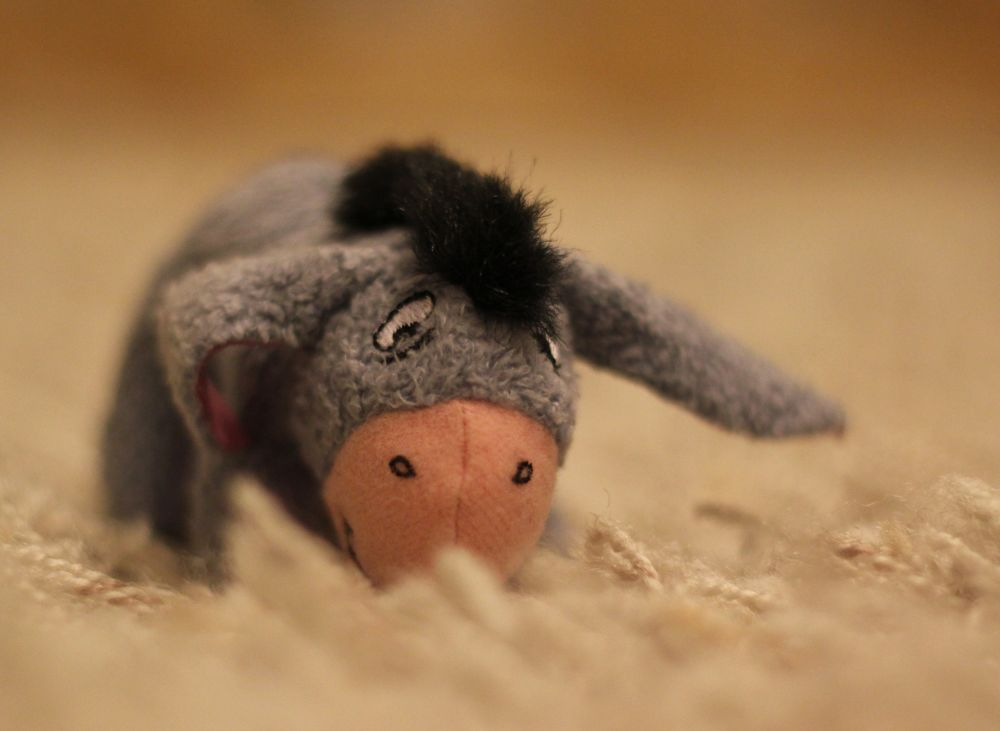
\includegraphics[width=9cm]{images/ihaa.jpg}
    \caption{Eeyore, or Ihaa, a very sad donkey.}
    \label{fig:eeyore}
  \end{center}
\end{figure}


% Comment: If your sentence ends in a capital letter, like here, you should
% write \@ before the period; otherwise LaTeX will assume that this is not
% really an end of the sentence and will not put a large enough space after the
% period. That is, LaTeX assumes that you are (for example), enumerating using
% capital roman numerals, like I. do something, II. do something else. In this
% case, the periods do not end the sentence.

% Similarly, if you do need a normal space after a period (instead of
% the longer sentence separator), use \  (backslash and space) after the
% period. Like so: a.\ first item, b.\ second item.

